% Unofficial University of Cambridge Poster Template
% https://github.com/andiac/gemini-cam
% a fork of https://github.com/anishathalye/gemini
% also refer to https://github.com/k4rtik/uchicago-poster

\documentclass[final]{beamer}

% ====================
% Packages
% ====================

\usepackage[T1]{fontenc}
\usepackage{lmodern}
\usepackage[size=custom,width=120,height=72,scale=1.0]{beamerposter}
\usetheme{gemini}
\usecolortheme{cam}
\usepackage{graphicx}
\usepackage{booktabs}
\usepackage{tikz}
\usepackage{pgfplots}
\pgfplotsset{compat=1.14}
\usepackage{anyfontsize}
\usepackage{xcolor,mdframed}

% ====================
% Lengths
% ====================

% If you have N columns, choose \sepwidth and \colwidth such that
% (N+1)*\sepwidth + N*\colwidth = \paperwidth
\newlength{\sepwidth}
\newlength{\colwidth}
\setlength{\sepwidth}{0.025\paperwidth}
\setlength{\colwidth}{0.3\paperwidth}
\setlength{\paperwidth}{48in}
\setlength{\paperheight}{36in}
\newcommand{\separatorcolumn}{\begin{column}{\sepwidth}\end{column}}

% ====================
% Title
% ====================

\title{Discover User-App Interactions \& \\  
Solutions to Reducing the Initial User-CPU Latency
}

\author{\LARGE{Thy Nguyen \and Milon Chakkalakal \and Pranav Thaenraj}}

\institute[shortinst]{\large{Advisors: Jamel Tayeb, Bijan Arbab, Sruti Sahani, Oumaima Makhlouk, Praveen Polasam, Chansik Im}}

% ====================
% Footer (optional)
% ====================

\footercontent{ \large{
  https://github.com/miloncl/System-Usage-Analysis \hfill
  UCSD HDSI - Intel \hfill
  {\{tcn002,mlonappa,ethaenra\}@ucsd.edu}}}
% (can be left out to remove footer)

% ====================
% Logo (optional)
% ====================

% use this to include logos on the left and/or right side of the header:
% \logoright{\includegraphics[height=7cm]{logo1.pdf}}
% \logoleft{\includegraphics[height=7cm]{logo2.pdf}}

% ====================
% Body
% ====================

\begin{document}

% Refer to https://github.com/k4rtik/uchicago-poster
% logo: https://www.cam.ac.uk/brand-resources/about-the-logo/logo-downloads
\addtobeamertemplate{headline}{}
{
    \begin{tikzpicture}[remember picture,overlay]
      \node [anchor=north west, inner sep=3cm] at ([xshift=0.0cm,yshift=0.75cm]current page.north west)
      {
\includegraphics[height=5.5cm]{HDSI_Intel.png}}; 
    \end{tikzpicture}

    \begin{tikzpicture}[remember picture,overlay]
      \node [anchor=north west, inner sep=3cm] at ([xshift=110.0cm,yshift=0.75cm]current page.north west)
      {
\includegraphics[height=5.5cm]{ucsd_logo.png}}; 
    \end{tikzpicture}
}

\begin{frame}[t]
\begin{columns}[t]
\separatorcolumn

\begin{column}{\colwidth}

  \begin{block}{\LARGE{Abstract}}

    \large{
    “Data loading” icons signal an unpleasant user wait experience and can tear people away from using an app. 
    This problem adversely affects user experience, but limited research has been done, 
    so we perform a study to collect user-app interaction data, analyze past behaviors to understand the user-wait events, 
    and propose solutions to reduce such waiting times. 
    Our study includes 2 phases: collecting data using Intel’s XLSDK and analyzing data using EDA, HMM, and LSTM/RNN.}

    \begin{figure}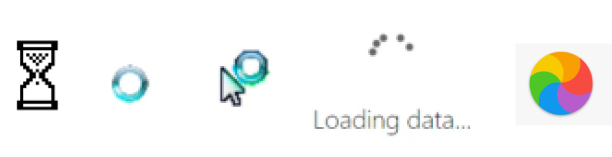
\includegraphics[width=0.6\textwidth, height=5cm]{user_wait.png}\end{figure}

  \end{block}

    \begin{alertblock}{\LARGE{Methodology of Data Collection}}

      \large{We write the \textbf{\textit{input libraries (ILs)}} using the  software development kit \textbf{\textit{XLSDK User Guide}}, along with the \textbf{\textit{Environment Server (ESRV)}}  toolchain  and the \textit{ \textbf{Intel® System Usage Report  (SUR)}} framework to anonymously gather and analyze data usage from multiple devices. The ILs include: 

    \begin{itemize}
      \item \textbf{Mouse Input IL}: capture the (X, Y) positions of the mouse in pixels (with or without noise)

      \item \textbf{User Wait IL}: retrieve the cursor type (e.g. loading or working smoothly) and its timestamp 

      \item \textbf{Mouse Hook IL}: track the UI objects clicked by the mouse

      \item \textbf{Foreground Window IL}: log the window's details detected by mouse clicks or time ticks

      \item \textbf{Desktop Mapper IL}: map all the open app windows in the z-order and store the relative position of an app on the screen as well as their individual size
    
    \end{itemize}

    We mainly focus on the data collected from the \textit{Foreground Window IL} for further exploration. }
    \begin{figure}
      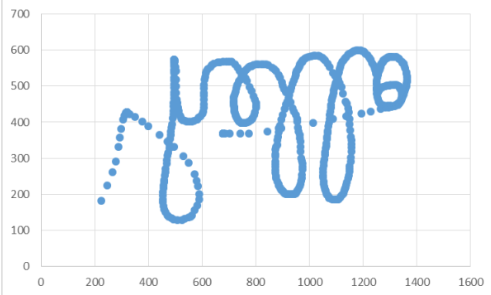
\includegraphics[width=0.475 \textwidth, height=11.5cm]{mouse_movement.png}
        \hspace{\fill}
        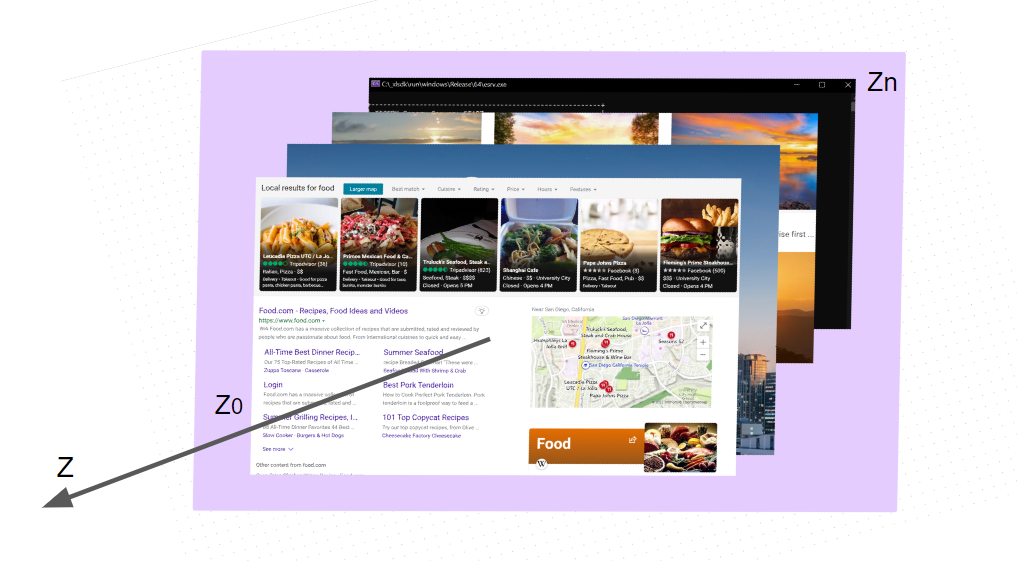
\includegraphics[width=0.475\textwidth, height=11.5cm]{foreground_desktopMapper.PNG}
      % \caption{\large{Mouse Movement, Foreground Window, and Z-axis}}\label{fig:xyz}
    \end{figure}
  \end{alertblock}

\begin{block}{\LARGE{Exploratory Data Analysis}}

  \begin{figure}
    \begin{mdframed}[backgroundcolor=gray!5,linecolor=gray!10]
    \centering{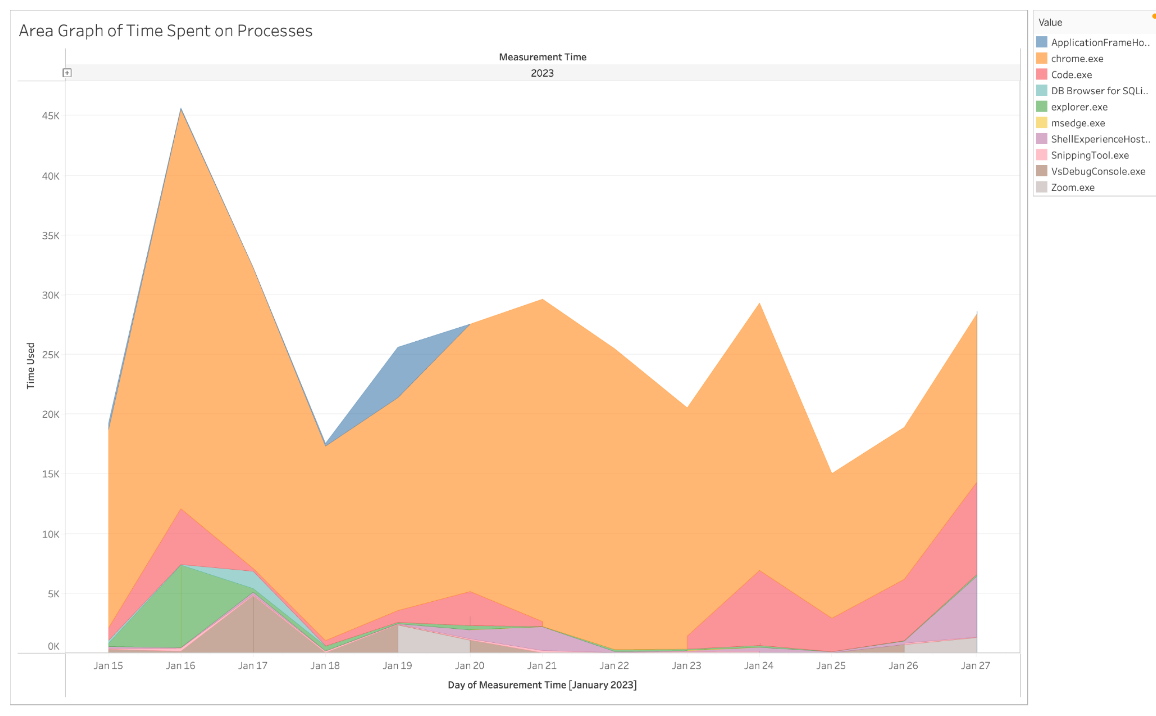
\includegraphics[width=0.96\textwidth, height=15cm]{time_spent.png}}
    \end{mdframed}
  \end{figure}

  \end{block}

\end{column}

\separatorcolumn

\begin{column}{\colwidth}

\begin{exampleblock}{\LARGE{Methodology of Predictive Tasks}}

  \large{\heading{Hidden Markov Model  (HMM)}

   \begin{itemize}
       \item \textbf{Problem Statement}: Predict the likelihood of using an app \textit{given} the former sequence of application usage
       \item \textbf{Basic Idea}: Utilize the conditional probability $P(A|B) = \frac{P(A\cap B)}{P(B)}$
       \item \textbf{HMM Assumptions}:
           
            1. \textbf{Markov Chain} Only the \underline{\textit{current}} state plays the most crucial role in predicting the future in the sequence; other states before that will not influence the future states 

            $$P(q_i = a | q_1q_2...q_{i-1}) = P(q_i= a | q_{i-1})$$

            where $q_k$ are the states for $k \in \{1, 2, ..., i\}$, e.g. hidden states \textit{chrome.exe} and \textit{explorer.exe}

           2. \textbf{Output Independence} The probability of observing an event $o_i$ only relies on the state $q_i$ that \underline{\textit{directly}} produced $o_i$. 
           
           $$P(o_i | q_1, ... q_i , ..., q_T, o_1, ..., o_i, ..., o_T) = P(o_i | q_i)$$
           
           where $o_1o_2...o_T$ is a sequence of T observations and $q_1, q_2 , ...,q_T$ are T states

        \item \textbf{Transition Matrix}:

        \item \textbf{Emission Matrix}: contains the emission probabilities, i.e. the likelihood of moving from one executable file to another app/tab. 
        
        \centering{$P($"chrome.exe" -> "Spotify"$)$ =  $P($"Spotify" | "chrome.exe"$)$}
       \end{itemize}
          
    \heading{Recurrent Neural Network (LSTM/RNN)}

    \begin{itemize}
       \item \textbf{Problem Statement}: Predict the (total) time usage of an app/tab/recorded process using the past \textit{time-series} data
       \begin{figure}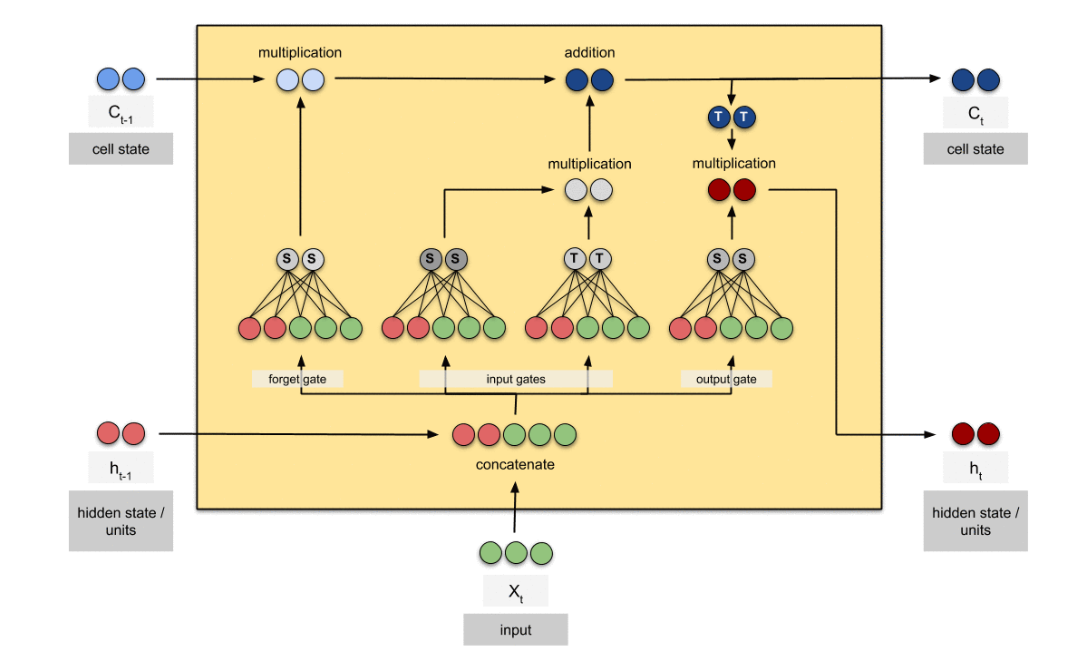
\includegraphics[width=0.95\textwidth, height=25cm]{lstm_1.png}\end{figure}

       \item \textbf{Feature Engineering}:
       
       1. Use time per day - split hourly between 24 columns (labeled 0 - 23)\\
       2. Lookback 3-5 time steps from the current timestamp\\
       3. One-hot-encoding(process names or weekdays); np.sin-encoding(hours)
       
       \item \textbf{Experiments}: implemented by \textit{Keras/Tensorflow}
      
       1. \textbf{Train/Test}: 80/20, no shuffle\\
       2. \textbf{Metrics}: RMSE, TP/TN/FP/FN, Preds==True if within 3 mins of real vals

      \end{itemize} }
    \end{exampleblock}

\end{column}

\separatorcolumn

\begin{column}{\colwidth}
  
\begin{block}
  {\LARGE{Prediction Results}}

  \large{
    \begin{table}
      \centering
      \begin{tabular}{l l l l}
        \toprule
        \multicolumn{1}{|l|}{\textbf{Model}} & \multicolumn{1}{|l|}{\textbf{Design (N=nodes)}} & \multicolumn{1}{|l|}{\textbf{Eval Bins}} & \multicolumn{1}{|l|}{\textbf{Performance}} \\
        \midrule
        
        \multicolumn{1}{|l|}{\begin{tabular}[c]{@{}l@{}}Vanilla LSTM \\  > Split Hourly \\ > OH(Process Name)\end{tabular}} &  
        \multicolumn{1}{|l|}{\begin{tabular}[c]{@{}l@{}}Input RNN (64N)\\ Hidden Dense (4N)\\ Output Dense(1N)\end{tabular}} & 
        \multicolumn{1}{|l|}{\begin{tabular}[c]{@{}l@{}}[0, 0.01] \\ (.01, .02]  \\ (.02, .2] \\ (.2, max] \end{tabular}} &  
        \multicolumn{1}{|l|}{\begin{tabular}[c]{@{}l@{}}TP = 691, TN = 0\\ FP = 65, FN = 0 \\ ACC = $\approx$ 91.4\% \end{tabular}} \\
        \midrule

        \multicolumn{1}{|l|}{\begin{tabular}[c]{@{}l@{}}Stacked LSTM \\  > Split Hourly \\ > OH(Process Name)\end{tabular}} &                                                                                                     
        \multicolumn{1}{|l|}{\begin{tabular}[c]{@{}l@{}}Input LSTM (16N)\\ Hidden LSTM (32N)\\ Hidden Dense (64N) \\ Output Dense(1N)\end{tabular}} & 
        \multicolumn{1}{|l|}{\begin{tabular}[c]{@{}l@{}}[0, 0.01] \\ (.01, .02]  \\ (.02, .2] \\ (.2, max] \end{tabular}} &  
        \multicolumn{1}{|l|}{\begin{tabular}[c]{@{}l@{}}TP = 467, TN = 52\\ FP = 13, FN = 224 \\ ACC = $\approx$ 68.65\% \end{tabular}} \\
        \midrule

        \multicolumn{1}{|l|}{\begin{tabular}[c]{@{}l@{}}Vanilla LSTM \\  > Split Hourly \\ > Lookback(3 timesteps)\end{tabular}} &  
        \multicolumn{1}{|l|}{\begin{tabular}[c]{@{}l@{}}Input LSTM (50N)\\ Output Dense(1N)\end{tabular}} & 
        \multicolumn{1}{|l|}{\begin{tabular}[c]{@{}l@{}}Preds==True \\ if abs(diff) <= 3mins \end{tabular}} &  
        \multicolumn{1}{|l|}{\begin{tabular}[c]{@{}l@{}} RMSE = 938.67 \\ ACC = $\approx$ 22.93\% \end{tabular}} \\
        \midrule
        
        \multicolumn{1}{|l|}{\begin{tabular}[c]{@{}l@{}}Stacked LSTM \\  > Split Hourly \\ > Lookback(5 timesteps)\end{tabular}} &                                                                                            
        \multicolumn{1}{|l|}{\begin{tabular}[c]{@{}l@{}}Input LSTM (50N)\\ Hidden LSTM (50N)\\ Output Dense(1N)\end{tabular}} & 
        \multicolumn{1}{|l|}{\begin{tabular}[c]{@{}l@{}}Preds==True \\ if abs(diff) <= 3mins \end{tabular}} &  
        \multicolumn{1}{|l|}{\begin{tabular}[c]{@{}l@{}} RMSE = 1134.68 \\ ACC = $\approx$ 27\% \end{tabular}} \\
        \midrule
                                                                              
        \bottomrule
      \end{tabular}
    \end{table}
  }
  

  \large{
    \begin{table}
      \centering
      \begin{tabular}{l l l l}
        \toprule
        \multicolumn{1}{|l|}{\textbf{Model}} & \multicolumn{1}{|l|}{\textbf{Design (N=nodes)}} & \multicolumn{1}{|l|}{\textbf{Eval Bins}} & \multicolumn{1}{|l|}{\textbf{Performance}} \\
        \midrule
        
        \multicolumn{1}{|l|}{\begin{tabular}[c]{@{}l@{}}Vanilla LSTM \\  > Split Hourly \\ > OH(Process Name)\end{tabular}} &  
        \multicolumn{1}{|l|}{\begin{tabular}[c]{@{}l@{}}Input RNN (64N)\\ Hidden Dense (4N)\\ Output Dense(1N)\end{tabular}} & 
        \multicolumn{1}{|l|}{\begin{tabular}[c]{@{}l@{}}[0, 0.01] \\ (.01, .02]  \\ (.02, .2] \\ (.2, max] \end{tabular}} &  
        \multicolumn{1}{|l|}{\begin{tabular}[c]{@{}l@{}}TP = 691, TN = 0\\ FP = 65, FN = 0 \\ ACC = $\approx$ 91.4\% \end{tabular}} \\
        \midrule

        \multicolumn{1}{|l|}{\begin{tabular}[c]{@{}l@{}}Stacked LSTM \\  > Split Hourly \\ > OH(Process Name)\end{tabular}} &                                                                                                     
        \multicolumn{1}{|l|}{\begin{tabular}[c]{@{}l@{}}Input LSTM (16N)\\ Hidden LSTM (32N)\\ Hidden Dense (64N) \\ Output Dense(1N)\end{tabular}} & 
        \multicolumn{1}{|l|}{\begin{tabular}[c]{@{}l@{}}[0, 0.01] \\ (.01, .02]  \\ (.02, .2] \\ (.2, max] \end{tabular}} &  
        \multicolumn{1}{|l|}{\begin{tabular}[c]{@{}l@{}}TP = 467, TN = 52\\ FP = 13, FN = 224 \\ ACC = $\approx$ 68.65\% \end{tabular}} \\
        \midrule

        \multicolumn{1}{|l|}{\begin{tabular}[c]{@{}l@{}}Vanilla LSTM \\  > Split Hourly \\ > Lookback(3 timesteps)\end{tabular}} &  
        \multicolumn{1}{|l|}{\begin{tabular}[c]{@{}l@{}}Input LSTM (50N)\\ Output Dense(1N)\end{tabular}} & 
        \multicolumn{1}{|l|}{\begin{tabular}[c]{@{}l@{}}Preds==True \\ if abs(diff) <= 3mins \end{tabular}} &  
        \multicolumn{1}{|l|}{\begin{tabular}[c]{@{}l@{}} RMSE = 938.67 \\ ACC = $\approx$ 22.93\% \end{tabular}} \\
        \midrule
        
        \multicolumn{1}{|l|}{\begin{tabular}[c]{@{}l@{}}Stacked LSTM \\  > Split Hourly \\ > Lookback(5 timesteps)\end{tabular}} &                                                                                            
        \multicolumn{1}{|l|}{\begin{tabular}[c]{@{}l@{}}Input LSTM (50N)\\ Hidden LSTM (50N)\\ Output Dense(1N)\end{tabular}} & 
        \multicolumn{1}{|l|}{\begin{tabular}[c]{@{}l@{}}Preds==True \\ if abs(diff) <= 3mins \end{tabular}} &  
        \multicolumn{1}{|l|}{\begin{tabular}[c]{@{}l@{}} RMSE = 1134.68 \\ ACC = $\approx$ 27\% \end{tabular}} \\
        \midrule
                                                                              
        \bottomrule
      \end{tabular}
    \end{table}
  }
  


  \end{block}
    \begin{block} {\LARGE{Conclusion}}

    \begin{itemize}
      \large{
      \item \textbf{Data Collection} 
      
      1.  \textcolor{brown}{\textit{Foreground Window IL}} provides the most applicable data for further analysis using EDA, HMM, RNNs \\
      2. Data should be collected \underline{\textit{continuously}} and \underline{\textit{consistently}} to allow detecting the patterns of user behaviors 
      \item \textbf{Predictive Tasks} 
      
      1. More data -> better predictive results \\
      2. Feature engineering, input RNN libraries, and hyperparameter tuning greatly influence the model performance \\
      3. We can use these results to infer the daily sequence of app usage and their use times --> devise solutions to reduce the initial user-CPU latency
    
      \item \textbf{Proposed Solutions}
      
      Using our predictive results, we can further develop a script to process the background tasks and utilize the \textit{Task Manager} to open the next app 2-3 mins beforehand \\
      }
      
    \end{itemize}
  \end{block}

  
  % \begin{block}{\LARGE{References}}

  %   \nocite{*}
  %   \footnotesize{\bibliographystyle{plain}\bibliography{poster}}

  % \end{block}

\end{column}

\separatorcolumn
\end{columns}
\end{frame}

\end{document}
